\documentclass[12pt]{article}
\usepackage{a4}
\usepackage[english]{babel}
\setlength{\parindent}{0.35cm}
\pagestyle{headings}
\usepackage{graphicx}
\usepackage{grffile}
%Multiple picture in one figure
%\usepackage{subfigure}
\usepackage{subfig}
\usepackage{listings}
\usepackage{color}
\usepackage{wrapfig}
%Floating-Umgebungen
\usepackage{float}
%Math-Environment
\usepackage{amsmath}
\usepackage{amssymb}
%Better SI-Units
\usepackage{siunitx}
%Using Appendix
\usepackage[title]{appendix}
%Using URL
\usepackage[hidelinks]{hyperref}
%Using Colored Tables
\usepackage{colortbl}
\newcommand{\gray}{\rowcolor[gray]{.90}}
\usepackage{esvect}
% Build fancy tables
\usepackage{booktabs}
%Configure geometry
\usepackage{geometry}
\geometry{
	a4paper,
	left=3cm,
	right=3cm,
	top=3cm,
	bottom = 3cm,
	}

\lstset{
	language=C++,
	basicstyle=\small\ttfamily,
	keywordstyle=\color{blue}\ttfamily,
	stringstyle=\color{red}\ttfamily,
	commentstyle=\color{green}\ttfamily,
	morecomment=[l][\color{magenta}]{\#},
}


\begin{document}
	
	\title{
		\textbf{\huge{CSE 446: Machine Learning Winter 2018 }} \\[2cm]
		\LARGE{Assignment 1}\\[1cm]
	}
	\author{from \\ Lukas Nies \\ University of Washington}
	\date{01/18/18}
	\clearpage\maketitle\thispagestyle{empty}
	\newpage

	\tableofcontents
	\setcounter{page}{0}
	\newpage
	
	% To start with section 1 labeled as section 0
	\setcounter{section}{-1}
	

\section{Policies}

\subsection{List of Collaborators}

\subsection{List of Acknowledgments}

\subsection{RTFM}

I have read and understood these policies.

\section{Problem: Criteria for Choosing a Feature to Split}

We build a tree with the dataset $D$ consisting $n$ negative examples (label 0) and $p$ positive examples (label 1). 

\subsection{Not Splitting}

If we are at the bottom of our decision tree and don't have any features left to split, consider the subset $D'$ of data $D$ with $n'$ negative and $p'$ positive examples. The smallest number of mistakes we can make in this subset is given by

\begin{align}
	\text{err}(D') = \min(n',p') = 
	\begin{cases}
		p' & \text{if } p'< n' \\
		n' & \text{if } n'< p'
	\end{cases}
\end{align}

The achieve the minimum the node must be labeled accordingly, with $1$ if $n'< p'$ or with $0$ if $n'> p'$. 

\subsection{Splitting}

Now we have a new feature $\Phi$ which splits the subsection $D'$ according to the contingency table:
% Table generated by Excel2LaTeX from sheet 'Sheet1'
\begin{table}[htbp]
	\centering
	\begin{tabular}{|c|c|c|}
		\toprule
		y     & \multicolumn{2}{c|}{$\Phi$} \\
		& \multicolumn{1}{c}{0} & 1 \\
		\cmidrule{2-3}    0     & $n_0$    & $n_1$ \\
		\cmidrule{2-3}    1     & $p_0$    & $p_1$ \\
		\bottomrule
	\end{tabular}%
	\caption{Contingency table for $\Phi'$}
	\label{tab:tabel1}%
\end{table}%
By splitting we generate two new sub-nodes: $(n_0,p_0)$ and $(n_1,p_1)$. The error for splitting is given by the sum of the errors of both nodes
\begin{align}
\text{err}(D') = \min(n_0,p_0) + \min(n_1,p_1),
\end{align}
where $n'=n_0 + n_1$ and $p'=n_1+p_1$. The error reduction rate ($\text{err}\_\text{red}$) is given by the reduction of error if comparing the error of "not splitting" with the error of "splitting", divided by the total number of examples in node $D'$:
\begin{align}
\text{\text{err}\_\text{red}}(D'): \frac{\min(n',p')-\left(\min(n_0,p_0) + \min(n_1,p_1)\right)}{\lvert D' \rvert}.
\end{align} 
Consider the maximal possible error (in this case for binary data) when $n'=p'=0.5 \lvert D' \rvert$
\begin{align}
\text{err}_\text{max}(D')=\min(n',p')=0.5\lvert D' \rvert,
\end{align}
then the maximal possible error reduction is given by 
\begin{align}
\text{\text{err}\_\text{red}}(D'): \frac{\min(0.5 \lvert D'\rvert,0.5 \lvert D' \rvert)-\left(\min(n_0,p_0) + \min(n_1,p_1)\right)}{\lvert D' \rvert} = 0.5,
\end{align}
where either $p_0=0$ or $n_0=0$ and $p_1=0$ or $n_1=0$ (maximal information gain).

\subsection{Mutual Information}

\begin{figure}[t!]
	\centering
	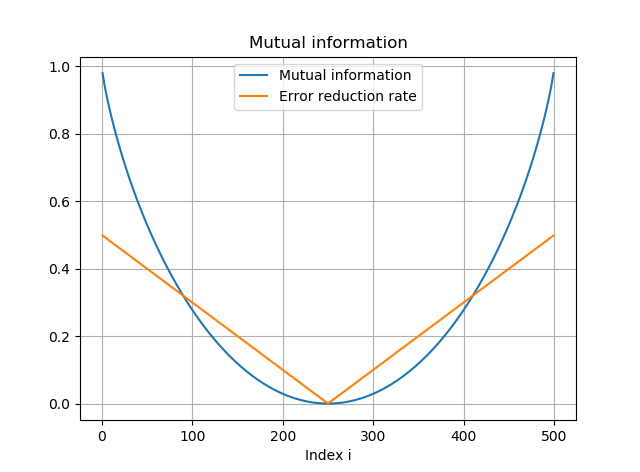
\includegraphics[width=0.65\linewidth]{../Problem_1/Figure_1.png}
	\caption{Comparison of mutual information between feature and label and error reduction rate for splitting the dataset.}
	\label{fig:1.3}
\end{figure}

The mutual information is a measure of information gain when splitting a dataset. In figure \ref{fig:1.3} the mutual information and the error reduction rate are plotted for problem $1.3$. Both functions are symmetric around index $250$ which represents equally distributed examples in form of $n_0=n_1=p_0=p_1=250$ . \par 
As we showed in the previous part of this problem, the error reduction rate is maximal for the case where the error of a node is $0$ after splitting. Corresponding to this the information gain in form of the mutual information is highest. \par
For increasing indices the information gain and the error reduction rate decrease until a minimum in $i=250$, afterwards rising again.    

\section{Decision Stumps and Trees}

\subsection{Built two decision stumps}

In figure \ref{fig:2.1} the comparison of of error rates and mutual information for different threshold splits and features are plotted. \par 
The top row shows the error as a function threshold. The feature "age" generates two minimums corresponding to two possible splits to minimize the error when splitting. For feature "salary" we get only one minimum but the error reduction is larger. \par 
The mutual information is plotted in the bottom row. Since the mutual information gives the information gain for a split we have to search for maximums. Both features give one maximal values which we can choose as a threshold to split the node. \par
In figure \ref{fig:stumps} the decision stumps are plotted for the best thresholds found in figure \ref{fig:2.1}. The error rate depends on choosing a feature to split and on the method to calculate the best threshold. An 

\begin{figure}[t!]
	\centering
	\subfloat[Error for the feature "age"] {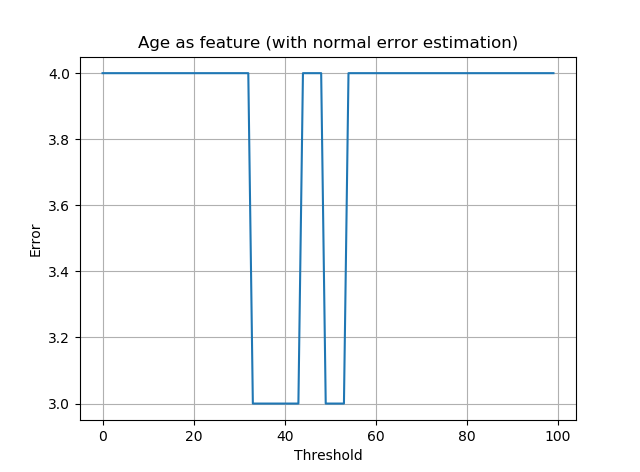
\includegraphics[width=0.45\textwidth]{../Problem_2/Figure_2.1_age_normal.png}}
	\hfill
	\subfloat[Error for the feature "salary"] {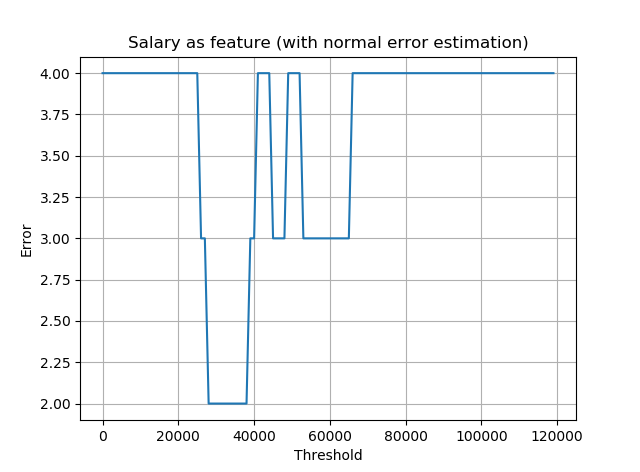
\includegraphics[width=0.45\textwidth]{../Problem_2/Figure_2.1_sal_normal.png}}
	\hfill
	\subfloat[Mutual information for the feature "age"] {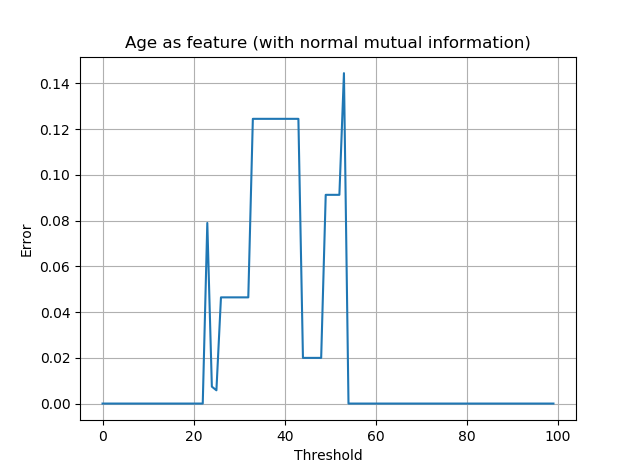
\includegraphics[width=0.45\textwidth]{../Problem_2/Figure_2.1_age_mut.png}}
	\hfill
	\subfloat[Mutual information for the feature "salary"] {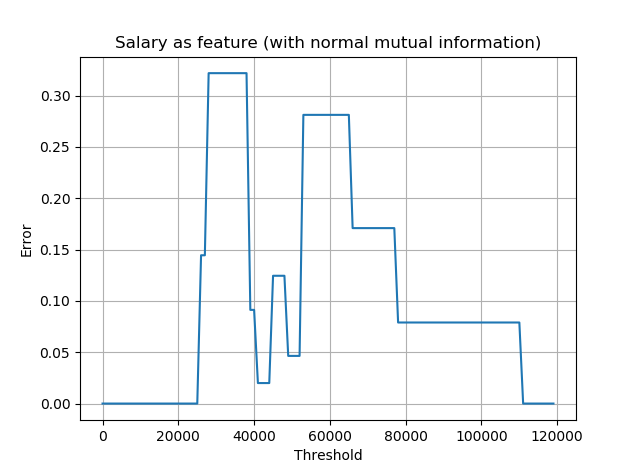
\includegraphics[width=0.45\textwidth]{../Problem_2/Figure_2.1_sal_mut.png}}
	\caption[]{Comparison of error rates and mutual information for different threshold splits and features. For generating this data a script has been written to scan through different thresholds with a fine reasonable step width. The error respectively mutual information was calculated as shown in problem 1. }
	\label{fig:2.1}
\end{figure}
\begin{figure}[h!]
	\centering
	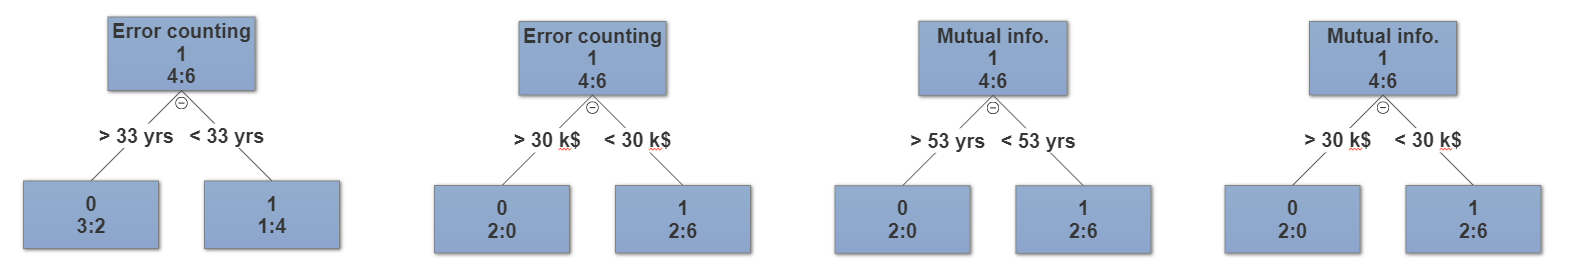
\includegraphics[width=1\linewidth]{../Problem_2/Figure_2.1_stamps.PNG}
	\caption{Decision stumps built after searching for the best threshold (Fig \ref{fig:2.1}).}
	\label{fig:stumps}
\end{figure}

\subsection{Build Decision Tree}

\begin{figure}[h]
	\centering
	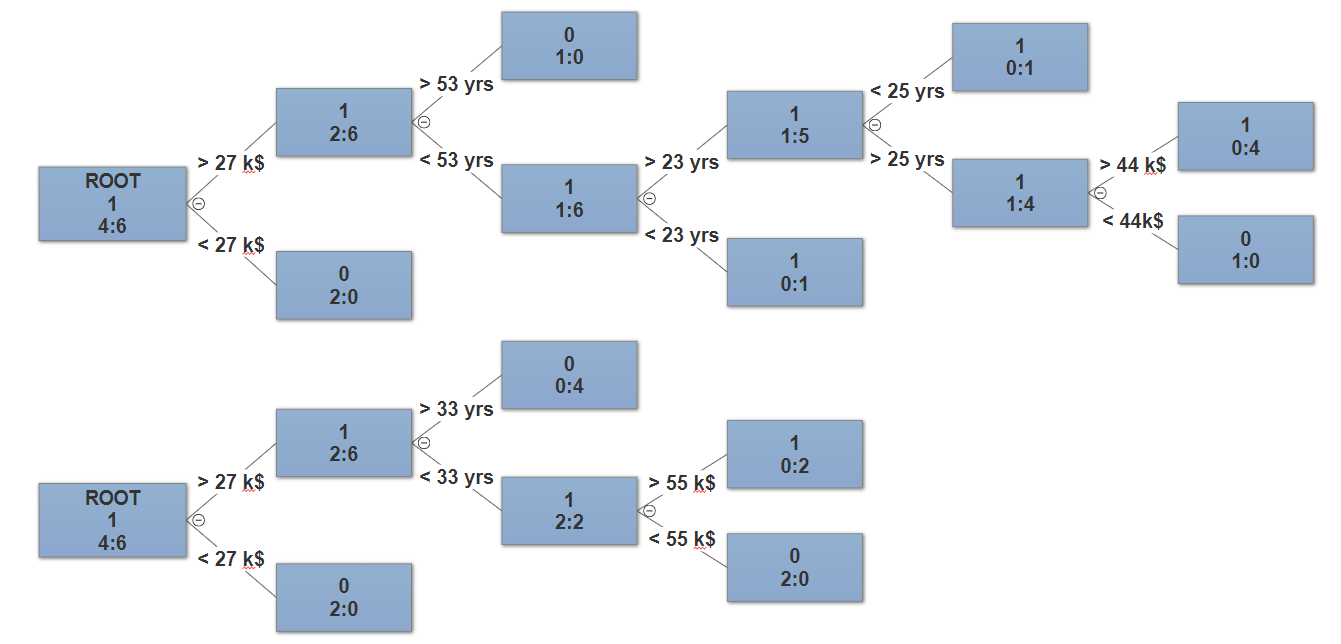
\includegraphics[width=1\linewidth]{../Problem_2/2.2.png}
	\caption{Greedily built decision trees. The splits for the upper tree were decided by searching for the best threshold to lower the total error. The splits for the lower tree were motivated by the best threshold corresponding to the largest information gain (mutual information). The label in the graphic for each node depicts the given label (upper row) and the abundance of negative examples (lower row, left value) and positive examples (lower row, right value). The errors for both trees are vanishing for deep nodes.}
	\label{fig:tree}
\end{figure}



In figure \ref{fig:tree} the greedily built decision trees are shown. We can see that the lower tree (built by using mutual information) only needs six nodes to reach an overall error of zero on the training set while the upper tree (built by counting errors) needs ten nodes. 

\subsection{Multivariate Decision Tree}

To built the multivariate decision tree we can utilize some of the basic geometric foundations used in the Perceptron algorithm. We have to learn the function
\begin{align}
f(\vec{x})=\left[\sum_{d=1}^{2}w_dx_d\right]-1=w_1x_\text{age}+w_2x_\text{salary}-1.
\end{align}
Since we work in two dimensions it's most convenient to just "guess" the hyperplane of the data which is in this case of dimension one, a line. Let $\vec{h}$ be the vector of this hyperplane. By drawing a straight line to separate negative and positive examples we can calculate the slope. This yields in 
\begin{align*}
\vec{h} = \begin{pmatrix}35 \\ 40000\end{pmatrix}
\end{align*}
where the first component corresponds to the age and the second component corresponds to the salary. According the the Perceptron the weight vector $\vec{w}$ is perpendicular to the hyperplane. To get $\vec{w}$ we can perform a rotation of $\vec{h}$ by applying a 2D rotation matrix:
\begin{align*}
\vec{w}=\text{rot}(90\degres)
\end{align*}

\subsection{Discussion}

\section{A "Baby" no Free Lunch Theorem}

Considering a function
\begin{align}
f:\{0,1\}^m\rightarrow \{0,1\}
\end{align}
mapping a binary string of length $m$ to a label, either $0$ or $1$. 

\subsection{The Number of Inputs}

The number of possible input strings is given by 
\begin{align}
N_\text{input}=2^m 
\end{align}
and for the length $m=5$ we have $32$ different input strings.

\subsection{The Number of Function}

The number of possible functions to map the input string to a label is given by:

\subsection{Obtaining low expected loss}

\subsection{Discussion}

\section{Implementation: \textit{K}-Means}
The script loops over $K \in \{1,2,\dots,10\}$, randomly initializes five times for each $K$ and returns the result with the lowest within-group sum of squares. 
\subsection{Putting it all Together}
\begin{figure}
	\centering
	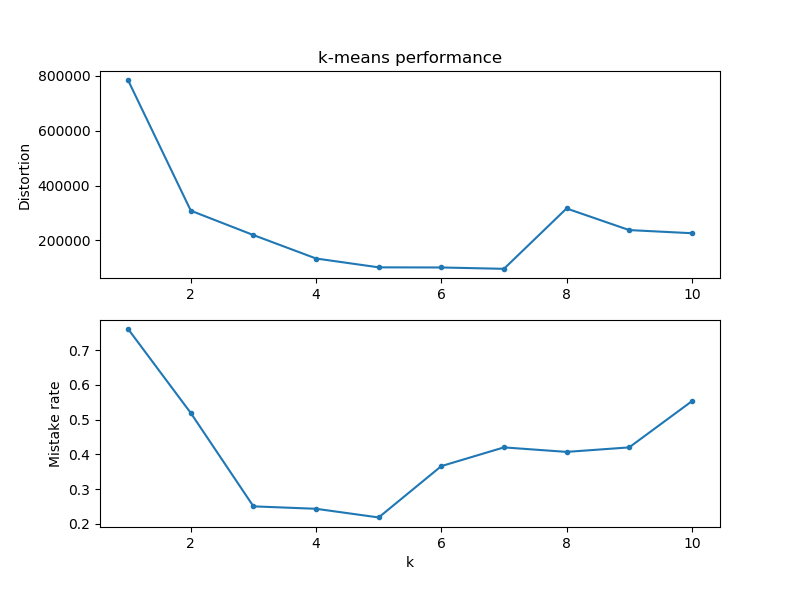
\includegraphics[width=\linewidth]{../Problem_4/Run_2.png}

\end{figure}



%\chapter*{Bibliography}
%\addcontentsline{toc}{chapter}{Bibliography}%	

\bibliographystyle{unsrt}
\bibliography{./bib}





\end{document}  